\begin{figure}[t]
\centering
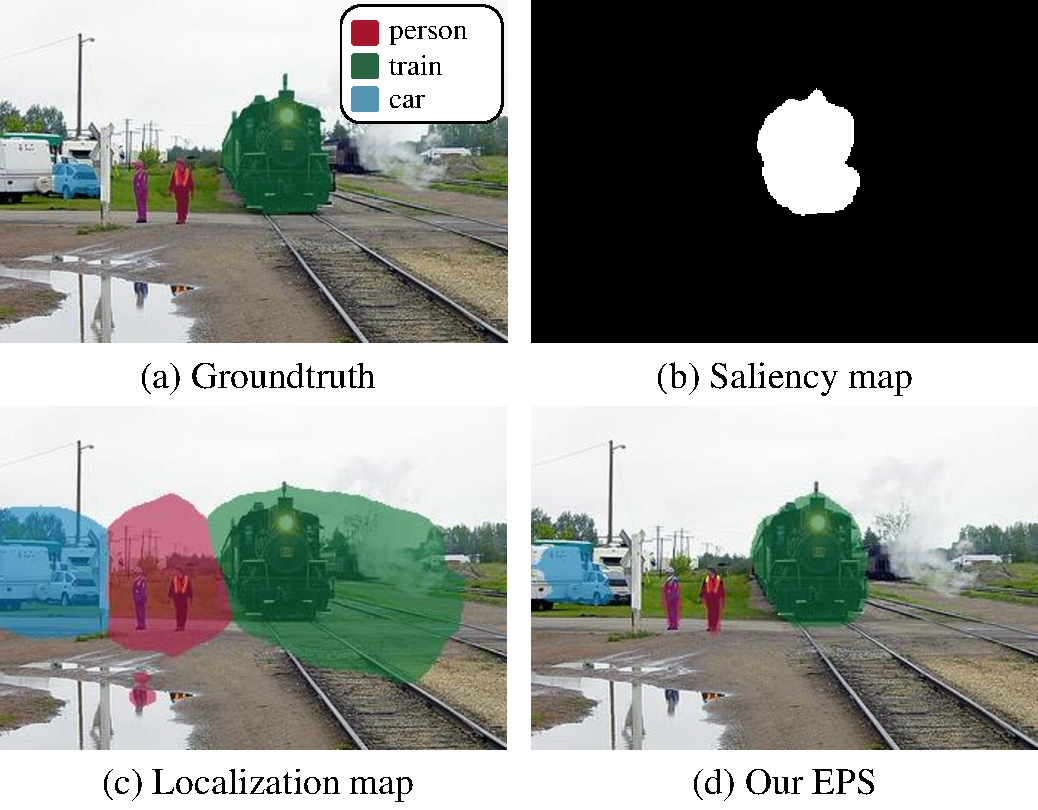
\includegraphics[width=8 cm]{figures/fig_concept.pdf}
\caption{WSSSのための顕著性マップとローカライゼーションマップの両方を利用する動機付けの例。(a) グラウンドトゥルース、(b) PFAN~\cite{zhao2019pyramid}による顕著性マップ、(c) CAM~\cite{zhou2016learning}によるローカライゼーションマップ、(d) 顕著性マップとローカライゼーションマップの両方を利用して分類器を訓練する我々のEPS。顕著性マップは\emph{人}と\emph{車}を捉えることができないが、我々の結果はそれらを正しく復元でき、ローカライゼーションマップは2つのオブジェクトを過剰に捉えていることに注意。} \vspace{-2mm}
\label{fig:concept}
\end{figure}
